
\section{SIFT algorithm explanation}

This section details the SIFT algorithm.
For reference,~\ref{eq:gaussian} shows the Gaussian function.
\begin{equation}
  \label{eq:gaussian}
  g(x) = \frac{1}{\sqrt{2*\pi*\sigma}}*e^{-x^2/2\sigma^2}
\end{equation}


\begin{easylist}
  \ListProperties(Progressive*=3ex, Space=0.15cm, Space*=0.15cm, Space1=0.5cm, Space1*=0.5cm)

# Scale-space extrema detection: The goal is to select regions with a minima
and maxima of difference-of-Gaussian. This is done with an image pyramid with
resampling between each level.

## The input image is convolved with the Gaussian function using
\(\sigma=\sqrt{2}\), which yields image A.\label{extrema:conv}

## Image A is then convolved again with
\(\sigma=\sqrt{2}\), resulting in image B with an effective smoothing of
\(\sigma=2\).\label{extrema:conv2}

## The difference-of-Gaussian is obtained by subtracting B from
A.\label{extrema:subs}

## The next level is obtained by sampling image B using bilinear interpolation,
with a pixel spacing of 1.5. This value is close enough to \(\sqrt{2}\), the
ratio between the Gaussians of A and B, but it gives a constant combination of
4 pixels, which is more efficient.\label{extrema:interp}

## Maxima and minima are obtained from the resulting image pyramid by comparing
each pixel to its neighbors.\label{extrema:compare1}

### First its compared to its 8 neighbors on the same level of the pyramid; If
it's an extrema (min or max) on that level, the closest pixel location is
calculated on the next lowest level of the pyramid.\label{extrema:compare2}

### If the pixel is lower or higher than this closest pixel and its 8
neighbors, the test is repeated for the level above.\label{extrema:compare3}

## After this procedure, we should have the key locations at maxima and minima
of difference-of-Gaussian in scale-space.

# Orientation assignment: The purpose of this step is to assign an orientation
to the found key points. This makes them more stable and invariant to scale and
rotation changes.\label{orientation:top}

## The orientation for a key location is gotten from a histogram of local image
gradient orientations. The histogram is created with a Gaussian weighted window
with a \(\sigma\) that is 3 times greater than the current smoothing
scale.\label{orientation:histogram1}

## The histogram has 36 bins that cover a full 360 degree range of
rotations.\label{orientation:histogram2}

## The histogram is smoothed prior to peak
selection.\label{orientation:histogram3}

# Keypoint descriptor: We want to make the found keypoints more robust against
small shifts in geometry.

## This is done by using the image gradients and orientations around the
keypoint, calculated for the orientation step.


## The gradients and orientations within 8 pixels of the keypoint are used. The
gradients are only taken in 8 directions, or orientation
planes.\label{keypoint1}

## The resulting gradients are smoothed because each one is an average of the
gradients of 8 pixels.\label{keypoint2}

## These orientations are then put into a histogram, which gives us the SIFT
feature vectors.\label{keypoint3}
\end{easylist}

\section{Annotated code}

\lstset{language=Matlab}

For brevity, I've only used step numbers to annotate the code. I used the code
found at \url{https://github.com/sun11/sw-sift}, because I couldn't get the
linked UCLA code to work. \\



Step~\ref{extrema:conv},\ref{extrema:conv2}
\begin{lstlisting}
% assume the original image has a blur of sigma = 0.5
input_img = gaussian(input_img,sqrt(init_sigma^2-0.5^2*4));


function [ out_img ] = gaussian( input_img, sigma )
% Function: Gaussian smooth for an image
k = 3;
hsize = round(2*k*sigma+1);
if mod(hsize,2) == 0
    hsize = hsize+1;
end
g = fspecial('gaussian',hsize,sigma);
out_img = conv2(input_img,g,'same');
end
\end{lstlisting}

Step~\ref{extrema:subs}
\begin{lstlisting}
% dog pyramid
dog_pyr = cell(octvs,1);
for i = 1:octvs
    dog_pyr{i} = zeros(gimg_size(i,1),gimg_size(i,2),s+2);
    for j = 1:s+2
    dog_pyr{i}(:,:,j) = gauss_pyr{i}(:,:,j+1) - gauss_pyr{i}(:,:,j);
    end
end
\end{lstlisting}

Step~\ref{extrema:interp},\ref{extrema:compare1},\ref{extrema:compare2},\ref{extrema:compare3}
\begin{lstlisting}
% width of border in which to ignore keypoints
img_border = 5;
% maximum steps of keypoint interpolation
max_interp_steps = 5;
% low threshold on feature contrast
contr_thr = 0.04;
% high threshold on feature ratio of principal curvatures
curv_thr = 10;
prelim_contr_thr = 0.5*contr_thr/intvls;
ddata_array = struct('x',0,'y',0,'octv',0,'intvl',0,'x_hat',[0,0,0],'scl_octv',0);
ddata_index = 1;
for i = 1:octvs
    [height, width] = size(dog_pyr{i}(:,:,1));
    % find extrema in middle intvls
    for j = 2:s+1
        dog_imgs = dog_pyr{i};
        dog_img = dog_imgs(:,:,j);
        for x = img_border+1:height-img_border
            for y = img_border+1:width-img_border
                % preliminary check on contrast
                if(abs(dog_img(x,y)) > prelim_contr_thr)
                    % check 26 neighboring pixels
                    if(isExtremum(j,x,y))
                        ddata = interpLocation(dog_imgs,height,width,i,j,x,y,img_border,contr_thr,max_interp_steps);
                        if(~isempty(ddata))
                            if(~isEdgeLike(dog_img,ddata.x,ddata.y,curv_thr))
                                 ddata_array(ddata_index) = ddata;
                                 ddata_index = ddata_index + 1;
                            end
                        end
                    end
                end
            end
        end
    end
end

function [ flag ] = isExtremum( intvl, x, y)
% Function: Find Extrema in 26 neighboring pixels
    value = dog_imgs(x,y,intvl);
    block = dog_imgs(x-1:x+1,y-1:y+1,intvl-1:intvl+1);
    if ( value > 0 && value == max(block(:)) )
        flag = 1;
    elseif ( value == min(block(:)) )
        flag = 1;
    else
        flag = 0;
    end
end
\end{lstlisting}

Step~\ref{orientation:top}
\begin{lstlisting}
% determines gaussian sigma for orientation assignment
ori_sig_factr = 1.5;
% number of bins in histogram
ori_hist_bins = 36;
% orientation magnitude relative to max that results in new feature
ori_peak_ratio = 0.8;
% array of feature
features = struct('ddata_index',0,'x',0,'y',0,'scl',0,'ori',0,'descr',[]);
feat_index = 1;
for i = 1:n
    ddata = ddata_array(i);
    ori_sigma = ori_sig_factr * ddata.scl_octv;
    % generate a histogram for the gradient distribution around a keypoint
    hist = oriHist(gauss_pyr{ddata.octv}(:,:,ddata.intvl),ddata.x,ddata.y,ori_hist_bins,round(3*ori_sigma),ori_sigma);
    for j = 1:2
        smoothOriHist(hist,ori_hist_bins);
    end
    % generate feature from ddata and orientation hist peak
    % add orientations greater than or equal to 80% of the largest orientation magnitude
    feat_index = addOriFeatures(i,feat_index,ddata,hist,ori_hist_bins,ori_peak_ratio);
end
\end{lstlisting}

Step~\ref{keypoint1},\ref{keypoint2}
\begin{lstlisting}
% number of features
n = size(features,2);
% width of 2d array of orientation histograms
descr_hist_d = 4;
% bins per orientation histogram
descr_hist_obins = 8;
% threshold on magnitude of elements of descriptor vector
descr_mag_thr = 0.2;
descr_length = descr_hist_d*descr_hist_d*descr_hist_obins;
local_features = features;
local_ddata_array = ddata_array;
local_gauss_pyr = gauss_pyr;
clear features;
clear ddata_array;
clear gauss_pyr;
clear dog_pyr;
parfor feat_index = 1:n
    feat = local_features(feat_index);
    ddata = local_ddata_array(feat.ddata_index);
    gauss_img = local_gauss_pyr{ddata.octv}(:,:,ddata.intvl);
% computes the 2D array of orientation histograms that form the feature descriptor
    hist_width = 3*ddata.scl_octv;
    radius = round( hist_width * (descr_hist_d + 1) * sqrt(2) / 2 );
    feat_ori = feat.ori;
    ddata_x = ddata.x;
    ddata_y = ddata.y;
    hist = zeros(1,descr_length);
    for i = -radius:radius
        for j = -radius:radius
            j_rot = j*cos(feat_ori) - i*sin(feat_ori);
            i_rot = j*sin(feat_ori) + i*cos(feat_ori);
            r_bin = i_rot/hist_width + descr_hist_d/2 - 0.5;
            c_bin = j_rot/hist_width + descr_hist_d/2 - 0.5;
            if (r_bin > -1 && r_bin < descr_hist_d && c_bin > -1 && c_bin < descr_hist_d)
                mag_ori = calcGrad(gauss_img,ddata_x+i,ddata_y+j);
                if (mag_ori(1) ~= -1)
                    ori = mag_ori(2);
                    ori = ori - feat_ori;
                    while (ori < 0)
                        ori = ori + 2*pi;
                    end
                    % i think it's theoretically impossible
                    while (ori >= 2*pi)
                        ori = ori - 2*pi;
                    end
\end{lstlisting}

Step~\ref{keypoint3}, continuing from above\dots
\begin{lstlisting}
                    o_bin = ori * descr_hist_obins / (2*pi);
                    w = exp( -(j_rot*j_rot+i_rot*i_rot) / (2*(0.5*descr_hist_d*hist_width)^2) );
                    hist = interpHistEntry(hist,r_bin,c_bin,o_bin,mag_ori(1)*w,descr_hist_d,descr_hist_obins);
                end
            end
        end
    end
    local_features(feat_index) = hist2Descr(feat,hist,descr_mag_thr);
end
% sort the descriptors by descending scale order
features_scl = [local_features.scl];
[~,features_order] = sort(features_scl,'descend');
% return descriptors and locations
descrs = zeros(n,descr_length);
locs = zeros(n,2);
for i = 1:n
    descrs(i,:) = local_features(features_order(i)).descr;
    locs(i,1) = local_features(features_order(i)).x;
    locs(i,2) = local_features(features_order(i)).y;
end
\end{lstlisting}


\section{Images from the test run}

\begin{figure}[H]
  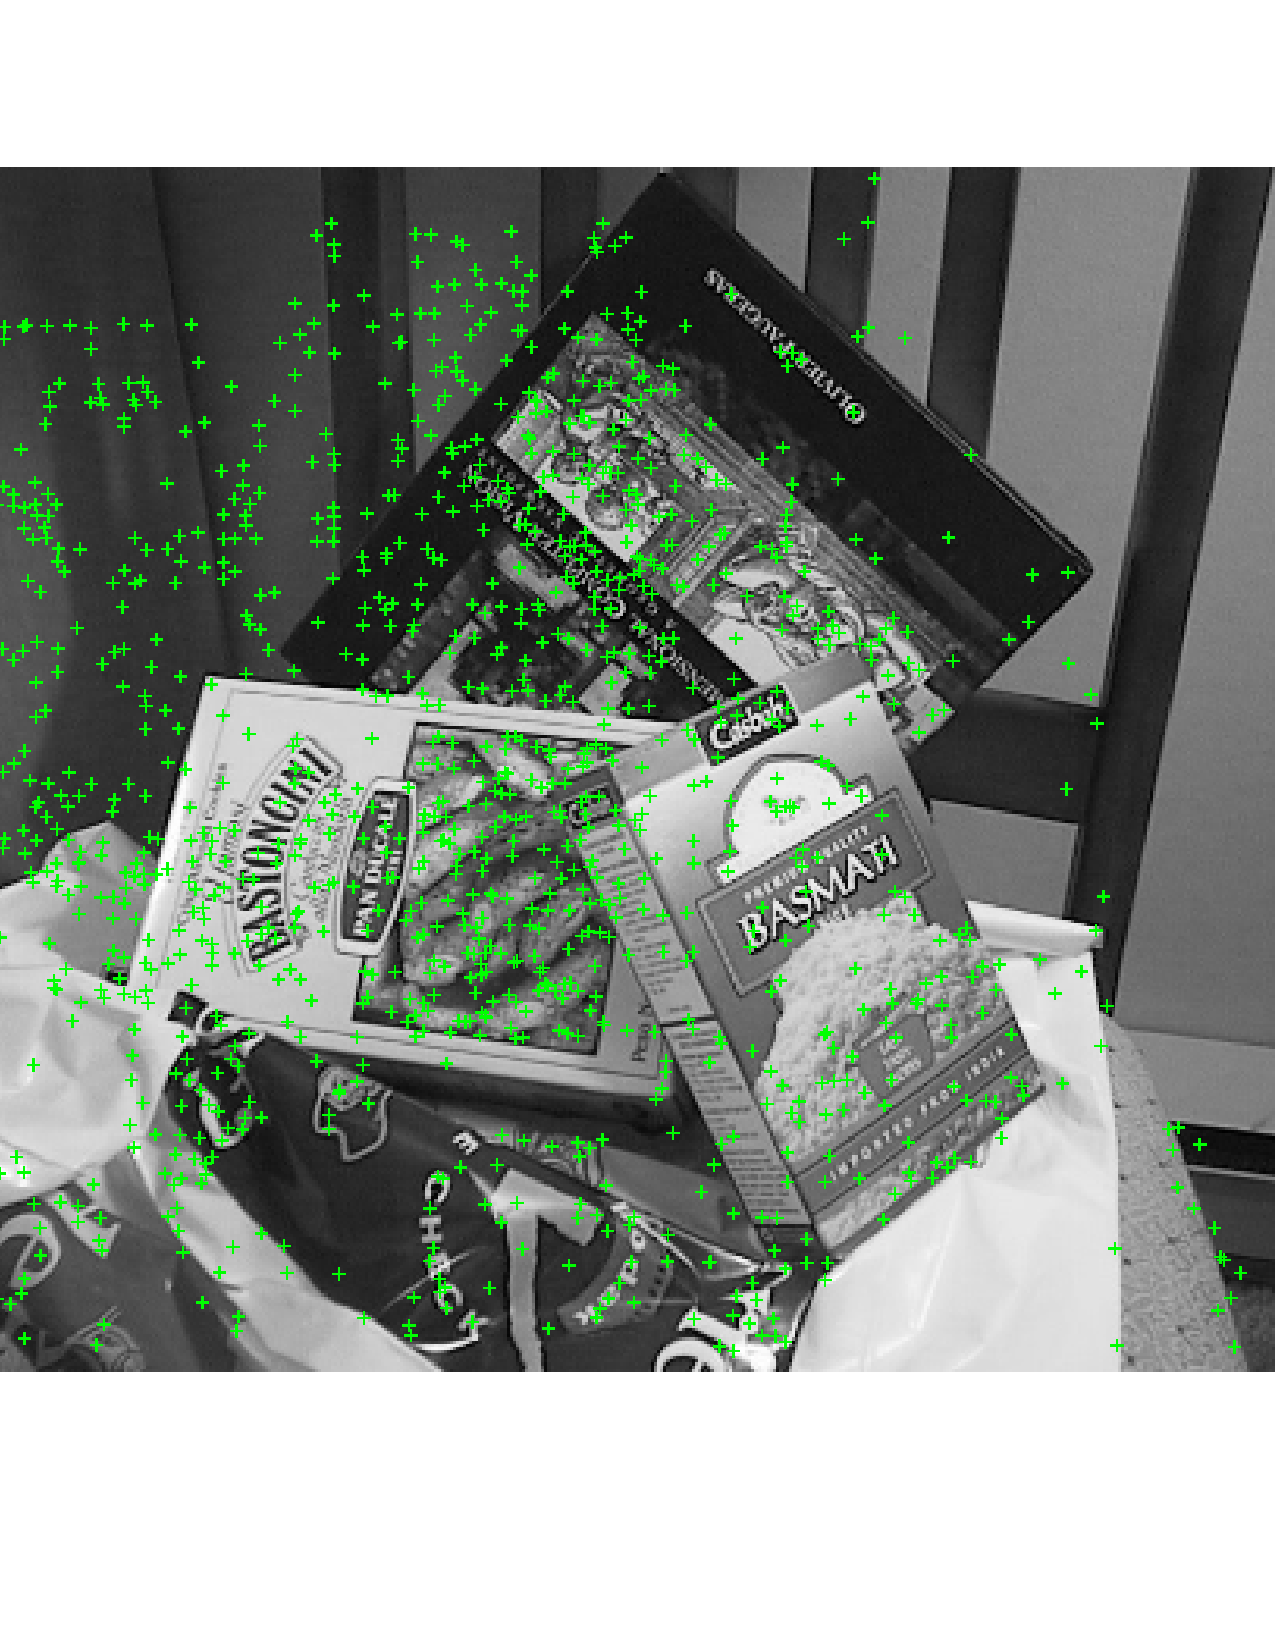
\includegraphics[width=0.5\textwidth]{img1}
  \caption{The first image with detected keypoints highlighted.}
\end{figure}

\begin{figure}[H]
  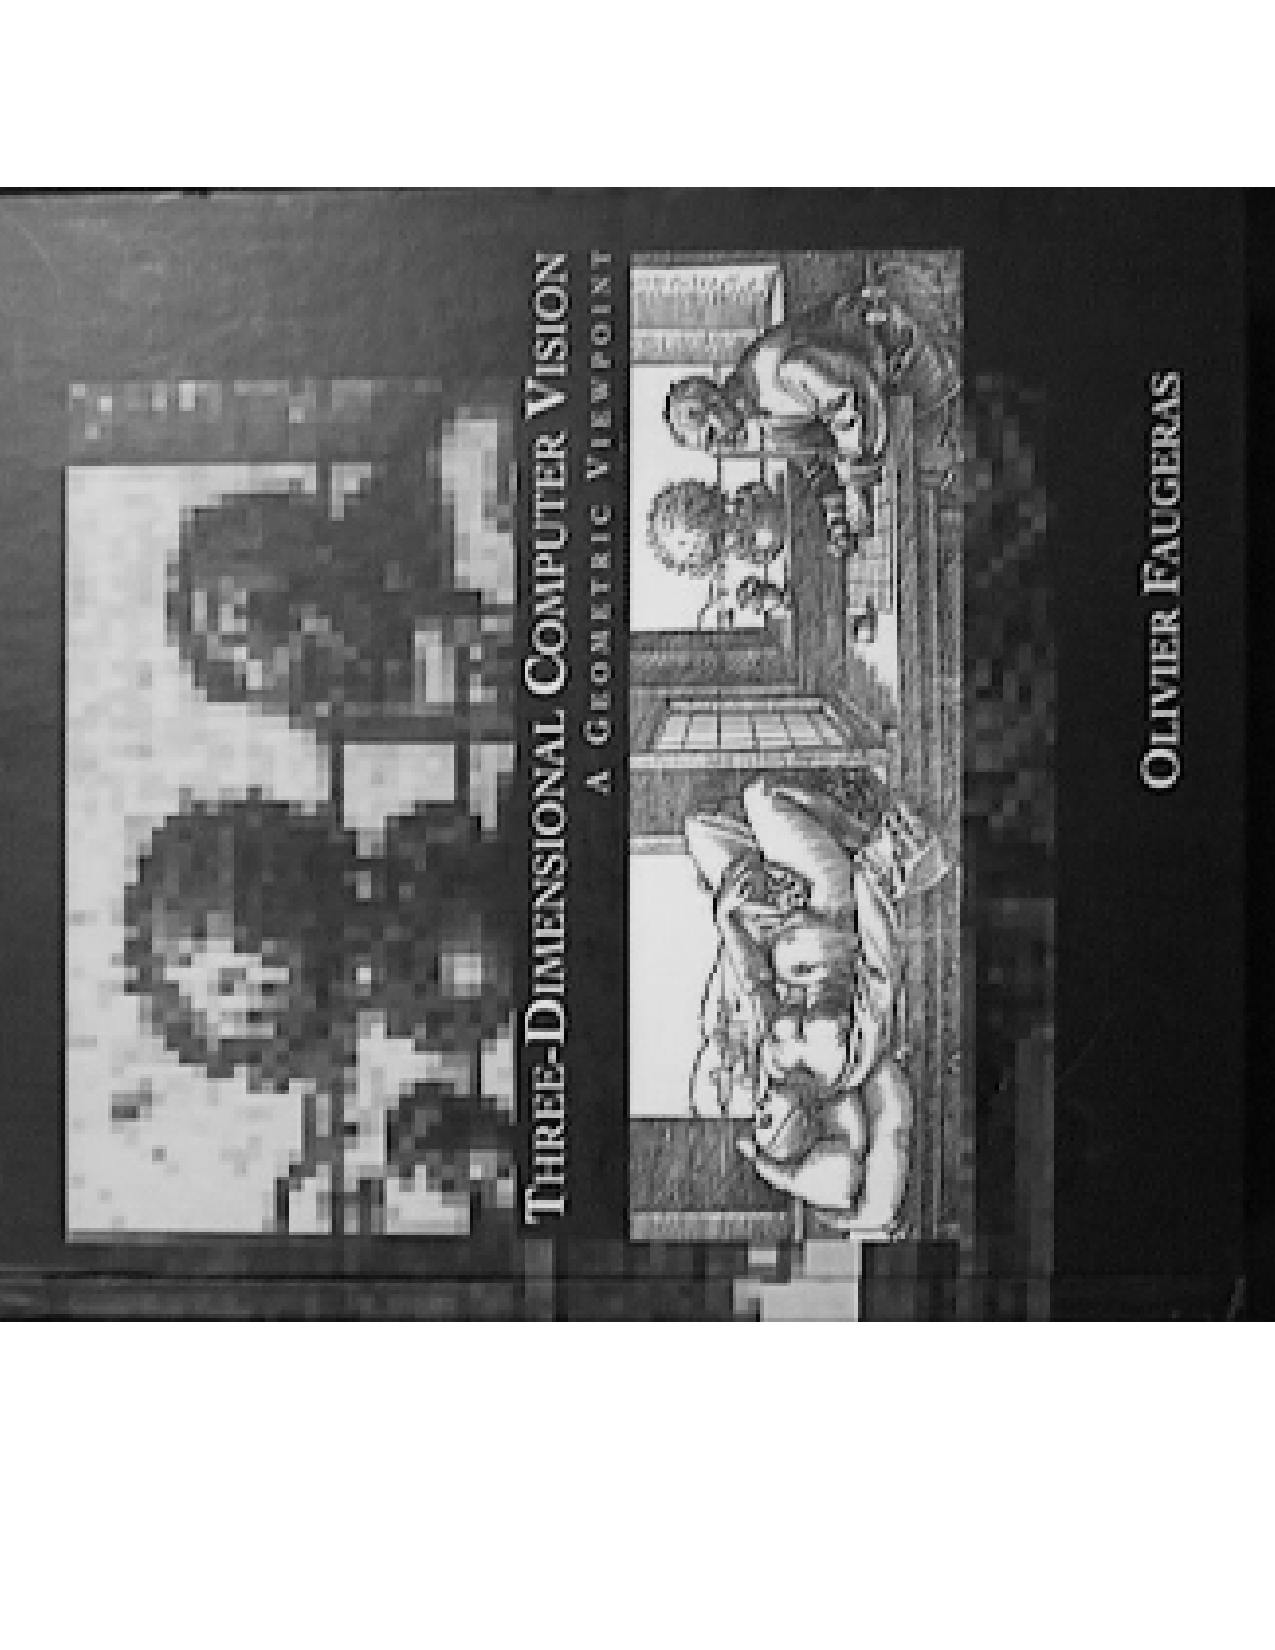
\includegraphics[width=0.5\textwidth]{img2}
  \caption{The second image with detected keypoints highlighted.}
\end{figure}

\begin{figure}[H]
  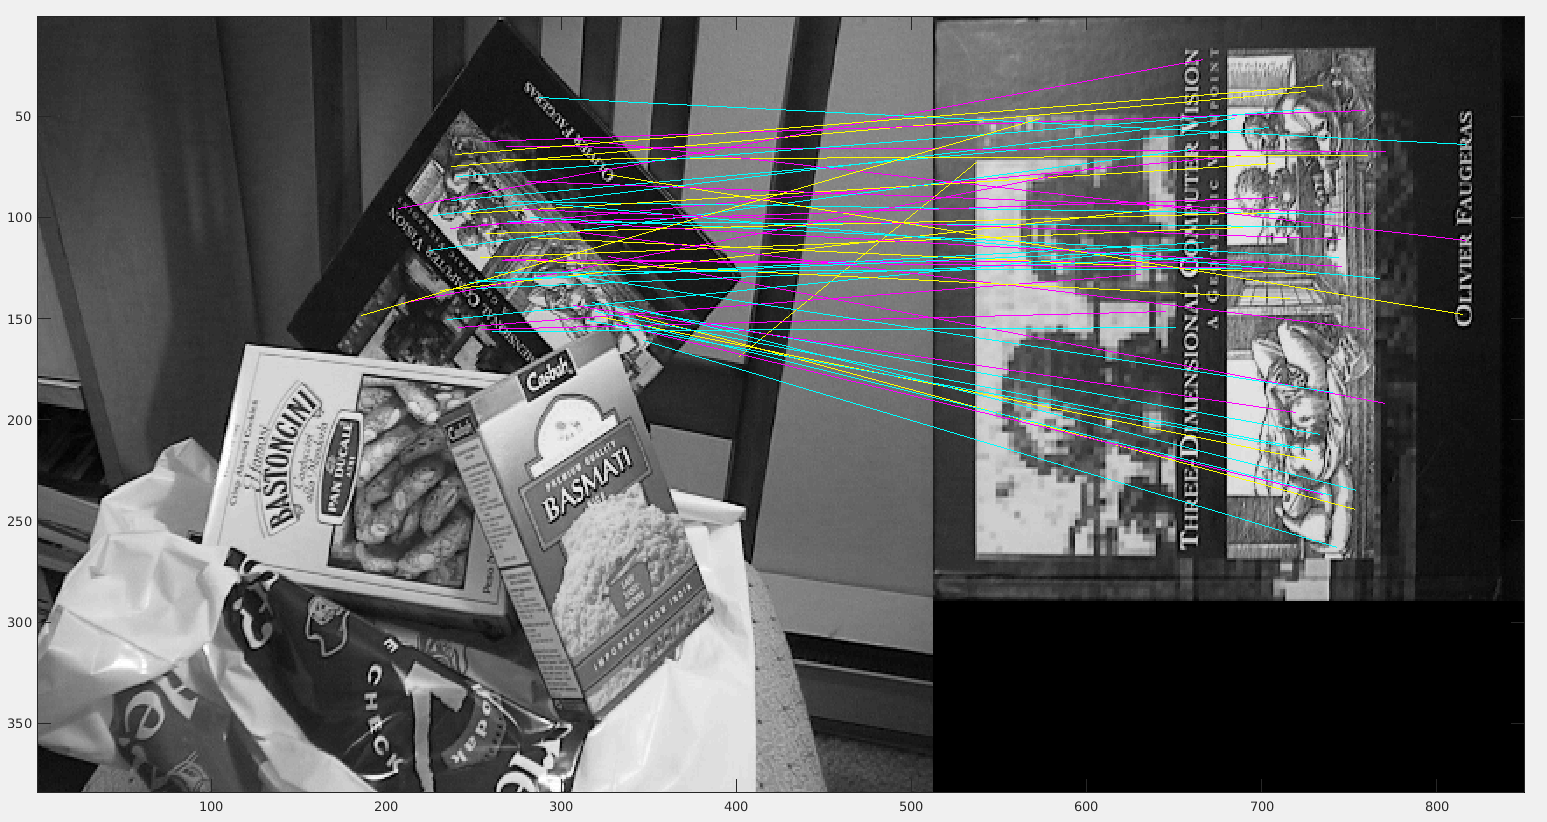
\includegraphics[width=1\textwidth]{matches}
  \caption{Detected matches between the two images.}
\end{figure}

